% !TEX encoding = UTF-8 Unicode
% -*- coding: UTF-8; -*-
% vim: set fenc=utf-8

\chapter{Arquitetura ARMFUL}%
\label{chap:arquitetura-armful}

Nesse capítulo é apresentada a arquitetura \abbrev{ARMFUL}{Analysis of Raw Data from Multiple Files} ARMFUL (do inglês: Analysis of Raw Data from Multiple Files; em tradução livre: Análise de Dados Científicos de Múltiplos Arquivos), introduzida recentemente em~\cite{silva2016situ,silva2017raw} pelo \abbrev{NACAD}{Núcleo Avançado de Computação de Alto Desempenho} Núcleo Avançado de Computação de Alto Desempenho (NACAD) da \abbrev{UFRJ}{Universidade Federal do Rio de Janeiro} UFRJ (Universidade Federal do Rio de Janeiro). Este capítulo também aborda o \textit{DfAnalyzer}, uma instância dessa arquitetura, implementada pelo mesmo laboratório.

\section{Visão geral}

A arquitetura \textbf{ARMFUL} tem suporte à extração de dados científicos, às técnicas de indexação e à análise de dados científicos a partir de múltiplos arquivos~\cite{silva2016situ} com o propósito de permitir o acesso direto a qualquer elemento ou região específica do espaço do fluxo de dados de uma simulação científica. Em outras palavras, ela permite a execução, \textit{off-line} e~/~ou \textit{on-line}\footnote{\textit{I.e.}, as consultas podem ser realizadas tanto \emph{após} as simulações científicas, quanto \emph{durante} as mesmas, respectivamente.}, de todos os três tipos de consultas apresentadas na \autoref{sec:tipos-de-consulta}. Essa flexibilidade e versatilidade na análise existe graças a uma \textbf{arquitetura de componentes}, que utiliza um banco de dados de proveniência para proporcionar um caminho de acesso entre o fluxo de dados e os dados científicos~\cite{silva2017raw}.

% Baseado na seção 5 de~\cite{silva2017raw}. Tentativa de tradução livre e de adaptação para o contexto desse trabalho.
A arquitetura ARMFUL funciona do seguinte modo: a gerência de conteúdos científicos é obtida a partir de dados científicos de arquivos, que então são correlacionados, em um repositório que é um SGBD relacional, através de dados de proveniência do seu respectivo fluxo de dados. Essa gerência de dados requer características que são específicas do domínio da simulação científica; por isso, modelos de dados de proveniência dessas simulações costumam ser representados em granularidade não-fina, \textit{i.e.}, as tabelas do SGBD possuem um grau de abstração relativamente alto para representar esses dados. Entretanto, consultas de proveniência possuem um valor analítico limitado caso não sejam relacionadas a elementos de dados específicos ao domínio da simulação computacional; contudo, esse relacionamento exige bastante esforço dos usuários de SGWfCs no que diz respeito a desenvolver, para cada domínio, um modelo de dados e programas científicos específicos para acessar, extrair e correlacionar os dados de domínio aos dados de proveniência. Nesse aspecto, a arquitetura ARMFUL contribui diminuindo o esforço necessário para capturar e representar esses dados de proveniência aravés da introdução e divisão de componentes genéricos e auto-contidos que modelam e correlacionam entre si, no mesmo banco de dados, (\(i\)) dados científicos específicos do domínio e (\(ii\)) proveniência.

Na \autoref{fig:armful-architecture-simplified}, podemos visualizar como é feita a representação e a divisão em componentes da arquitetura ARMFUL, que são os seguintes:

\begin{itemize}
    \item Banco de dados de proveniência;
    \item Extração de dados científicos;
    \item Indexação de dados científicos;
    \item Ingestão de dados de proveniência; e
    \item Processamento de consultas.
\end{itemize}

\begin{figure}[ht]
    \centering
    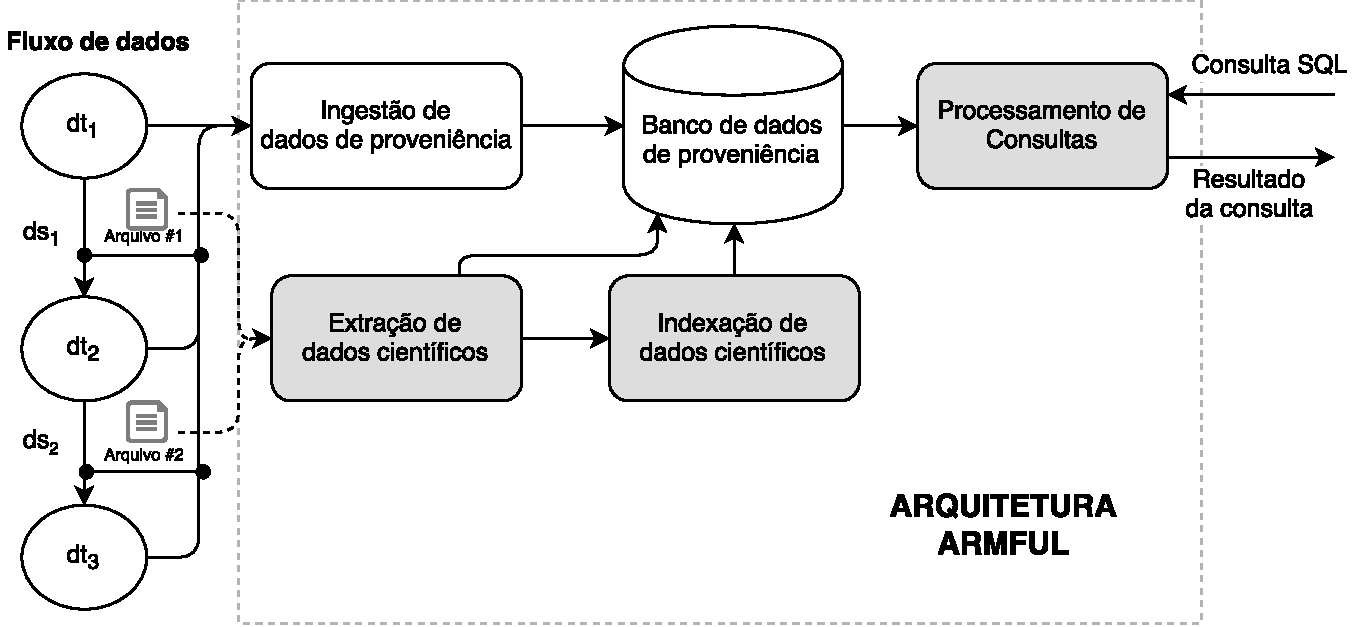
\includegraphics[width=\textwidth]{img/armful-architecture-simplified}
    \caption[Componentes da arquitetura ARMFUL]{Componentes da arquitetura ARMFUL. A cor branca representa as etapas relacionadas aos dados de proveniência, e a cor cinza tem relação com os dados científicos. Baseada em~\cite{silva2017raw}.}%
    \label{fig:armful-architecture-simplified}
\end{figure}

Os componentes na cor branca correspondem à captura e ao armazenamento de dados de proveniência em um banco de dados de proveniência. Em contrapartida, os componentes na cor cinza descrevem os passos responsáveis por: (\(i\)) extrair dados científicos de arquivos, (\(ii\)) gerar índices para os mesmos e (\(iii\)) permitir a consulta de proveniência \textbf{e} dados científicos a partir do mesmo banco de dados. Nas próximas subseções os componentes serão detalhados.

% Baseado na seção 5.1 de~\cite{silva2017raw}.
\subsection{Banco de dados de proveniência}%
\label{subsec:banco-de-dados-de-proveniencia}

O \textbf{banco de dados de proveniência}, que funciona como um repositório para os dados de proveniência, deve ser um \textbf{SGBD relacional}, e é responsável por armazenar, gerenciar e correlacionar (\(i\)) dados de proveniências e (\(ii\)) dados científicos, a fim de se beneficiar do suporte analítico de consultas do fluxo de dados. Além disso, SGBDs possuem solidez, confiabilidade e segurança, oriundas de uma experiência de mais de 30 anos de estudos científicos e aplicações no mundo real, provendo estratégias e algoritmos bem conhecidos que garantem atomicidade, consistência, isolamento e durabilidade (ACID) em transações, além de possuir soluções consolidadas e robustas no que diz respeito a recuperação de dados e controle concorrente de acesso~\cite{ozsu2011principles}.

\subsection{Extração e indexação de dados científicos}%
\label{subsec:extracao-e-indexacao-de-dados-cientificos}

O \textbf{componente de extração de dados científicos} tem o objetivo de ler o conteúdo de arquivos científicos, analisá-lo e então recuperar parte do conteúdo selecionado que é relevante de acordo com os atributos especificados pelo usuário. Para que esse objetivo seja completado, quatro etapas devem ser seguidas:

\begin{itemize}
    \item \textbf{leitura do conteúdo}: acesso aos arquivos científicos e leitura do seu conteúdo;
    \item \textbf{tokenização}: investigação de metadados relacionados à especificação do formato de arquivo, visando verificar se os dados científicos obtidos na etapa anterior correspondem ao domínio da simulação computacional processada atualmente;
    \item \textbf{filtragem de conteúdo}: a especificação do usuário é responsável por definir e restringir o que deve ser analisado e armazenado no banco de dados de proveniência, isto é, essa etapa evita armazenar atributos desnecessários, que não serão utilizados na próxima etapa;
    \item \textbf{análise}: conversão de cada dado científico filtrado em uma estrutura de dados apropriada para ser armazenada no SGBD.
\end{itemize}

O \textbf{componente de indexação de dados científicos} é opcional e visa indexar um conteúdo específico dos arquivos científicos a fim de agilizar o tempo de acesso direto a determinadas regiões do espaço de dados científicos através da gerência de metadados correlacionados ao fluxo de dados. A criação de índices é realizada segundo um algoritmo de indexação previamente definido, \textit{e.g.} indexação por \textit{bitmap} ou indexação posicional.

O volume de dados científicos que é gerado durante a execução de uma simulação computacional é um fator determinante para a definição da melhor estratégia para a representação desses dados~\cite{silva2015propostadoutorado}: em simulações que geram um pequeno volume de dados em cada transformação de dados e que possuem poucos atributos, a extração e ingestão (\textit{i.e.}, carga no banco de dados de proveniência) de dados científicos \emph{diretamente} com seus próprios valores de dados costuma ser uma abordagem melhor. Em contrapartida, em um cenário no qual um grande volume de dados --- com estruturas de dados complexas --- precisa ser capturado, o componente de indexação é fortemente recomendado.

\subsection{Ingestão de dados}%
\label{subsec:ingestao-de-dados}

O \textbf{componente de ingestão de dados} é responsável por coletar a \textbf{proveniência} do fluxo de dados, selecionando, manipulando e armazenando (\textit{i.e.} realizando a carga dos valores assumidos pelos atributos) convenientemente as informações referentes aos arquivos e dados científicos no banco de dados mencionado na \autoref{subsec:banco-de-dados-de-proveniencia}~\cite{silva2015propostadoutorado}. Em outras palavras, esse componente é responsável por alimentar e popular o SGBD com informações de dados de proveniência que serão posteriormente utilizadas para auxiliar o componente de processamento de consultas, que será discutido na próxima seção. Esse componente interfaceia diretamente com todo item do fluxo de dados.

A captura de dados de proveniência deve ser realizada com uma granularidade fina, de modo a apoiar e capturar os dois tipos de análises exploratórias em arquivos de dados científicos mencionadas na \autoref{subsec:categorias-de-dados-de-proveniencia} (proveniência prospectiva e retrospectiva). Além disso, também deve realizar a gerência do fluxo de dados nos níveis físico e lógico.

\subsection{Processamento de consultas}

Uma vez que todos os dados científicos e toda a proveniência sejam devidamente capturadas e armazenadas em um repositório SGBD, os usuários poderão consultá-los para apoiar (refutar ou validar) suas hipóteses científicas~\cite{silva2015propostadoutorado}. Nesse contexto, o \textbf{componente de processamento de consultas} é responsável por prover um mecanismo de consultas à proveniência e aos dados científicos armazenados em um banco de dados de proveniência compatível com um modelo de dados adequado. O comportamento desse componente é variável, dependendo da estratégia utilizada nos componentes anteriores --- de extração e de indexação. Uma vez que esse componente utiliza um SGBD para o armazenamento dos dados de proveniência, somente tipos de consultas que são permitidas e disponíveis pelo SGBD podem ser realizadas. Em particular, e como consequência disso, as consultas são comumente especificadas em uma linguagem de alto nível, como a linguagem declarativa SQL.

O processador de consultas é um componente bastante importante, já que é a principal interface entre os usuários e uma instância da arquitetura ARMFUL, e todas as consultas ao banco de dados são iniciadas (e especificadas) a partir dele.

\section{DfAnalyzer: uma instância da arquitetura ARMFUL}%
\label{sec:dfanalyzer-uma-instancia-da-arquitetura-armful}

\subsection{Visão Geral}%
\label{subsec:dfanalyzer-visao-geral}

Como vimos na seção anterior, a arquitetura ARMFUL é uma \textbf{abstração} que define e especifica componentes a fim de prover um mecanismo capaz de realizar consultas a um banco de dados, cujos dados de proveniência, execução e domínio foram oriundos de uma simulação computacional. Dito isso, o \textbf{DfAnalyzer} é uma \textbf{instância da arquitetura ARMFUL}; em outras palavras, ele consiste em uma implementação dessa arquitetura. Ele foi originalmente introduzido em~\cite{silva2016situ}. Os principais componentes do DfAnalyzer são abordados nas próximas subseções.

\subsection{Provenance Data Gatherer (PDG)}

O \textbf{Provenance Data Gatherer} (PDG) é o componente do DfAnalyzer responsável por \textbf{capturar dados de proveniência} (\textit{c.f.} \autoref{subsec:ingestao-de-dados}) assim como dados específicos do domínio a partir do código fonte da aplicação, gerando um arquivo JSON com o conteúdo extraído e as suas respectivas dependências de dados~\cite{silva2016situ}. Após a captura, a proveniência e os dados de domínio são carregados em um banco de dados que é compatível com um esquema (do inglês \textit{schema}) pré-definido e que é gerenciado pelo SGBD MonetDB~\cite{boncz2008breaking}, que consiste em um banco de dados orientado a colunas compatível com a linguagem SQL.

O motivo do MonetDB ter sido escolhido como o SGBD para a gerência e o armazenamento dos dados de proveniência deve-se principalmente ao fato do mesmo ser orientado e otimizado para a consulta de dados através de colunas --- diferentemente da maioria dos SGBDs tradicionais, como o MySQL e o SQLite, que são orientados a linhas. Isso é importante pois, em geral, o principal interesse nas consultas das simulações computacionais consiste na obtenção de apenas um subconjunto dos atributos presentes.
% https://www.monetdb.org/Documentation/Manuals/SQLreference/Indices
Além disso, o MonetDB trata suas cláusulas de indexação de forma peculiar e dinâmica: diferentemente de SGBDs tradicionais, essas cláusulas são postergadas, interpretadas meramente como \textit{hints}, sendo o MonetDB o responsável por tomar as decisões finais de manutenção e de criação de índices, visando assim acelerar o posterior acesso aos dados~\cite{url:monetdb}.

Existem duas fontes de proveniência para o PDG. Uma é a \textit{libMesh-sedimentation solver}, mencionada anteriormente na \autoref{subsec:dfanalyzer-visao-geral}, que contribui com dados de domínio obtidos diretamente do código fonte do resolvedor de dinâmica de fluidos computacionais. A outra é o ParaView Catalyst~\cite{ayachit2015paraview}, que é uma biblioteca com o qual o DfAnalyzer pode comunicar-se para aproveitar-se dos dados gerenciados em memória por ele e relacioná-los com o banco de dados de proveniência, além de prover recursos de visualização e de processamento de dados. O Paraview Catalyst pode ser utilizado para extrair dados que estão em memória, complementando a \textit{libMesh-sedimentation} e gerar visualizações de regiões de interesse.

\subsection{Raw Data Extractor (RDE)}

Uma vez que o PDG especializa-se em coletar proveniência e dados de domínio, o \textbf{Raw Data Extractor} (RDE) o complementa, sendo o componente responsável por \textbf{extrair} os dados científicos que estão presentes em arquivos científicos (\textit{c.f.} \autoref{subsec:extracao-e-indexacao-de-dados-cientificos}). Esses arquivos usualmente mantêm seus dados em formato binário, total ou parcialmente, sendo responsabilidade do RDE a leitura, filtragem e análise do conteúdo desses dados, transformando-os em um formato adequado para ser armazenado nos tipos e tabelas disponíveis no MonetDB. Dependendo da aplicação e da simulação científica, o conteúdo desses arquivos científicos pode ser ora armazenado diretamente no SGBD, ora armazenado indiretamente, através de ponteiros (referências de arquivos), ou estruturas de dados em formatos intermediários de representação.

\subsection{Raw Data Indexer (RDI)}

O \textbf{Raw Data Indexer} (RDI) é o componente do DfAnalyzer responsável por indexar dados científicos presentes em arquivos, com o objetivo de permitir o acesso eficiente aos dados durante a execução das consultas pelos usuários, diminuindo o tempo médio delas (\textit{c.f.} \autoref{subsec:extracao-e-indexacao-de-dados-cientificos}). O RDI é comumente utilizado para indexar estruturas de dados mais complexas, como matrizes e malhas esparsas, que demandam um custo de tempo para a carga de dados em uma base de dados muito grande. Outro fator para o uso de técnicas de indexação consiste na dificuldade de representar determinadas estruturadas de dados em um SGBD, por exemplo. Entretanto, esse trabalho não contempla o uso do RDI nos experimentos realizados, nem requer uma descrição detalhada desse componente, pois a implementação de indexação de dados científicos não foi considerada para o desenvolvimento do processador de consultas deste projeto de graduação.

\subsection{Query Processor (QP)}

O \textbf{Query Processor} (QP) é o componente responsável por auxiliar os usuários a \textbf{submeterem consultas} na linguagem SQL ao banco de dados de proveniência~\cite{silva2016situ}, realizar a validação dessas consultas --- por exemplo, se a sintaxe e~/~ou se os nomes dos atributos de dados estão corretos --- e então finalmente retornar e exibir os resultados das mesmas. Com o objetivo de facilitar a execução de consultas por novos usuários, sem a necessidade de que eles tenham que aprender todos os aspectos da sintaxe da linguagem SQL, uma nova forma simplificada de especificação e de descrição de consultas foi desenvolvida, a qual traduz e converte a consulta do usuário para SQL, e é essa conversão que é enviada ao MonetDB, o qual retorna os resultados para o usuário.

Essa conversão possui duas vantagens básicas: a primeira, mencionada anteriormente, é a facilidade para novos usuários interagirem com o DfAnalyzer, de forma mais intuitiva e direta, sem a necessidade de descrever uma consulta em SQL completa e válida, e nem a necessidade de conhecer completamente todos os dados do domínio. A segunda é a possibilidade do QP realizar otimizações na consulta antes de enviá-la diretamente ao MonetDB. Por exemplo, em dada consulta, a cláusula \textsc{FROM} pode ser otimizada, filtrando tabelas que não sejam realmente necessárias na consulta em questão, diminuindo a sobrecarga ao SGBD e recuperando apenas os dados realmente necessários para o sucesso da consulta.

O QP é capaz de realizar todos os três tipos de consultas mencionados anteriormente na \autoref{sec:tipos-de-consulta}: \((i)\) análise de dados científicos isolados de um único arquivo; \((ii)\) rastreamento de fluxos de múltiplos arquivos relacionados; e \((iii)\) rastreamento de elementos de dados relacionados e múltiplos arquivos. 
A principal contribuição deste trabalho encontra-se especificamente na implementação deste componente, a qual será detalhadamente discutida no \autoref{chap:rastros-de-proveniencia}.